\documentclass{beamer}

\usepackage{neuralnetwork}
\usepackage{anyfontsize}
\usepackage{pgfpages}

\usepackage{ragged2e} %文本两端对齐 \justifying
% \usepackage{tikz}
%\usetikzlibrary{matrix,chains,positioning,decorations.pathreplacing,arrows}

\setcounter{tocdepth}{2} % hide subsubsection in tableofcontents
\usetheme[hideothersubsections,numbers,sidebarshades]{Radboud}

% no indenting
\setlength{\parindent}{0pt}

% frame style
\AtBeginSection[]{
    \begin{frame}
    \frametitle{Outline}
    \tableofcontents[currentsection]
    \end{frame}
}

% beamer settings
\setbeamertemplate{footline}{}
\setbeamertemplate{sidebar left}[sidebar theme]
\setbeamercovered{transparent}
%\setbeameroption{show notes on second screen=right}
%\setbeamerfont{note page}{size=\tiny}
%\setbeameroption{show notes}
%\setbeameroption{show only notes}
\setbeameroption{hide notes}
\setbeamertemplate{itemize item}[circle]
\setbeamertemplate{subitemize item}[-]

\setbeamercovered{dynamic}
\setbeamerfont{author}{family=\rmfamily}



\begin{document}

    \title{\emph{The Report about CirCNN }}%题目
    \author[by Tianma Shen]{authors: Tianma Shen\\[5pt]\scriptsize{University of Shanghai for Science and Technology}}%作者
    % \date{}
    % disable sidebar content
    \setbeamertemplate{sidebar left}{}

    \begin{frame}
        \titlepage
    \end{frame}


    \begin{frame}
        \frametitle{Outline}%修改Outline的名字,一般不会动这个
        \tableofcontents
    \end{frame}

    
    % enable sidebar content
    \setbeamertemplate{sidebar left}[sidebar theme]

    \section{Background and Motivation}

    % ===== insert sections here =====

    \frame{
\frametitle{Background }%此页的标题

\begin{itemize}

	\item \justifying Large-scale deep neural networks (DNNs)

	\item Limitations of computer performance

	\item Difficult tasks with big data

\end{itemize}

}

    \frame{
\frametitle{Motivation}%此页的标题

\begin{itemize}

	\item \justifying Reduce weight storage (model size)

	\item Accelerate the computation

	\item Maintain accuracy

\end{itemize}

}
    %\input{...}

    % ================================
    \section{Novelty of CirCNN}

    \frame{
\frametitle{Novelty of CirCNN}%此页的标题

\begin{itemize}

	\item \justifying Supporting both FC and CONV layers

	\item Block-circulant matrices

\end{itemize}

}

    \section{Related Knowledge}

    
\frame{
\frametitle{Full Connect Layers}%此页的标题

\begin{center}
	\begin{neuralnetwork}[height=4]
		\newcommand{\nodetextclear}[2]{$a_#2$}
		\newcommand{\nodetextx}[2]{$x_#2$}
		\newcommand{\nodetexty}[2]{}
		\inputlayer[count=4, bias=false, title=Layer L, text=\nodetextx]
		\hiddenlayer[count=5, bias=false, title=Layer L+1, text=\nodetextclear] \linklayers
		\outputlayer[count=4, title=Layer L+2, text=\nodetexty] \linklayers
	\end{neuralnetwork}
\end{center}

\begin{eqnarray}
	% a_{5} &=& f\left( W_{51}\cdot X_{1}+W_{52}\cdot X_{2}+W_{53}\cdot X_{3}+W_{54}\cdot X_{4}\right)\\
	a_{1} &=& f\left( W_{11}\cdot X_{1}+W_{12}\cdot X_{2}+W_{13}\cdot X_{3}+W_{14}\cdot X_{4}\right)\\
	a_{5} &=& f\left( W_{51}\cdot X_{1}+W_{52}\cdot X_{2}+W_{53}\cdot X_{3}+W_{54}\cdot X_{4}\right)
\end{eqnarray}

}



    \frame{
\frametitle{Convolution Layer}%此页的标题

\begin{figure}
	\begin{center}
		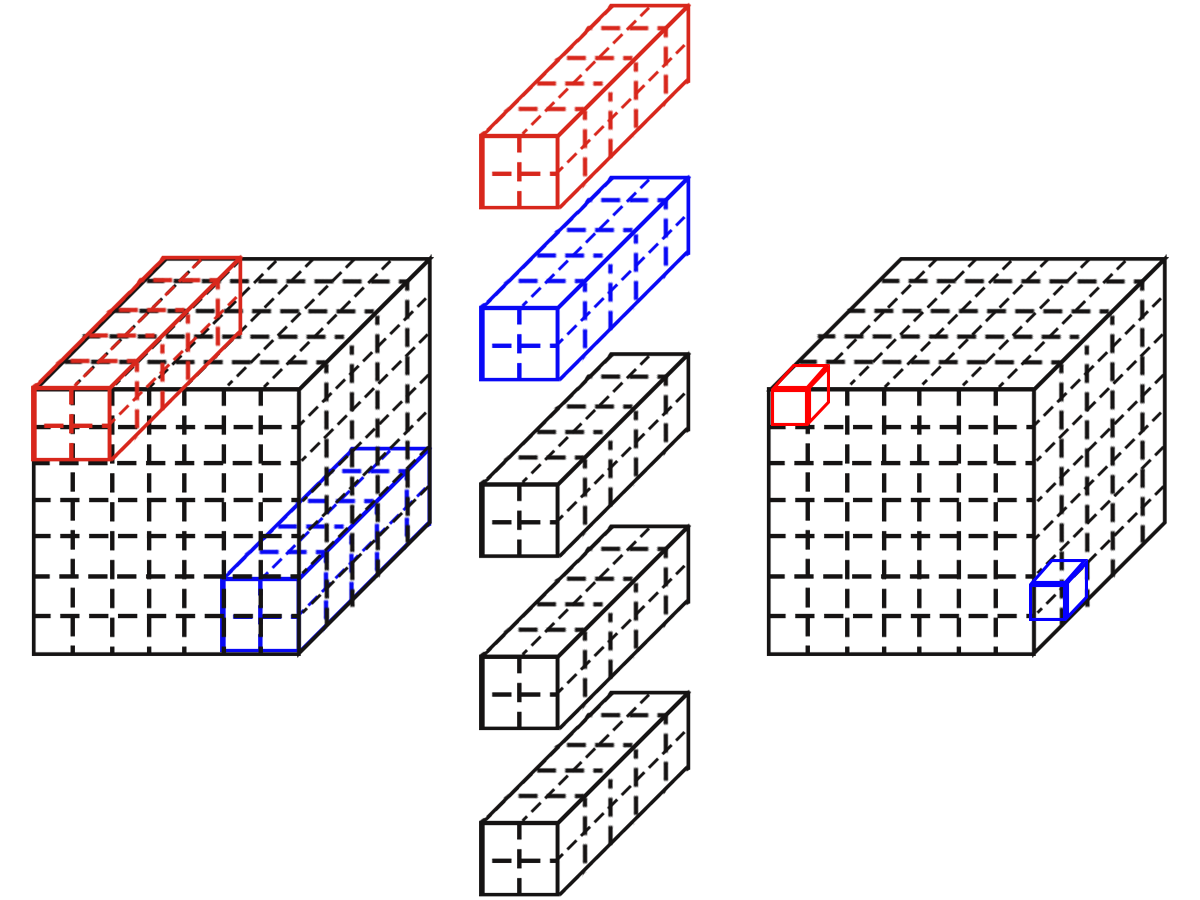
\includegraphics[width=0.7\linewidth]{Picture/conv.png}
		% \caption{Knowledge Graph of Machine Learning}
		% \label{Fig:1}
	\end{center}
	% \vspace{-0.1em}
\end{figure}

\begin{eqnarray}
	% a_{5} &=& f\left( W_{51}\cdot X_{1}+W_{52}\cdot X_{2}+W_{53}\cdot X_{3}+W_{54}\cdot X_{4}\right)\\
	Y\left( x,y,p\right) =\sum ^{r}_{i=1}\sum ^{r}_{j=1}\sum ^{c}_{c=1}F\left( i,j,c,p\right) X\left( x+i-1,y+j-1,c\right)
\end{eqnarray}

}
    \frame{
\frametitle{Circulant matrices}%此页的标题
\begin{eqnarray}
	\begin{bmatrix}
		W_{11}    &W_{12}   & W_{13}    & ... &W_{1n-2}  & W_{1n-1}  &W_{1n}  \\ 
		W_{1n}    &W_{11}   &W_{12}     & W_{13} & ... &W_{1n-2}  & W_{1n-1} \\ 
		W_{1n-1}  &W_{1n}   &W_{11}     &W_{12}  & W_{13} & ... &W_{1n-2}\\ 
		 .&  &  &  &  &  &.\\ 
		 .&  &  &  &  &  &. \\ 
		 .&  &  &  &  &  &. \\ 
		W_{13}    & ...     &W_{1n-2}   & W_{1n-1}  &W_{1n}    & W_{11} &W_{12}\\
		W_{12}    & W_{13}  & ...       &W_{1n-2}  & W_{1n-1}  &W_{1n}  & W_{11} 
	\end{bmatrix}
\end{eqnarray}
}
    \frame{
\frametitle{Discrete Fourier Transform}%此页的标题

\qquad The discrete Fourier transform transforms a sequence of N numbers $x_{0},x_{1},\ldots ,x_{N-1}$ into another sequence of complex numbers, $X_{0},X_{1},\ldots ,X_{N-1}$ ,which is defined by
\begin{eqnarray}
	% a_{5} &=& f\left( W_{51}\cdot X_{1}+W_{52}\cdot X_{2}+W_{53}\cdot X_{3}+W_{54}\cdot X_{4}\right)\\
	X_{k} &=& \sum ^{N-1}_{n=0}x_{n}\cdot e^{-i 2\pi k\dfrac {n}{N}}\\
	      &=& \sum ^{N-1}_{n=0}x_{n}\left[ \cos \left( 2\pi k\dfrac {n}{N}\right) -i\cdot \sin \left( 2\pi k\dfrac {n}{N}\right) \right] 
\end{eqnarray}

\qquad where the last expression follows from the first one by Euler's formula.

\qquad The transform is sometimes denoted by the symbol $\mathcal {F}$, as in $\mathbf {X} = \mathcal {F}\left\{\mathbf {x} \right\}$or $\mathcal {F}\left(\mathbf {x} \right)$ or $\mathcal {F}\mathbf {x}$.

}
    \frame{
\frametitle{Convolution theorem}%此页的标题

\qquad Let $\mathcal {F}$ denote the Fourier transform operator, so $\mathcal {F}\{f\}$ and $\mathcal {F}\{g\}$ are the Fourier transforms of $f$ and $g$, respectively. Then
\begin{eqnarray}
	% a_{5} &=& f\left( W_{51}\cdot X_{1}+W_{52}\cdot X_{2}+W_{53}\cdot X_{3}+W_{54}\cdot X_{4}\right)\\
	\mathcal {F} \left\{f * g\right\} &=& \mathcal {F} \left\{f  \right\} \cdot \mathcal {F} \left\{g\right\}\\
	f * g  &=& \mathcal {F}^{-1}\left\{\mathcal {F} \left\{f  \right\} \cdot \mathcal {F} \left\{g\right\}\right\}
\end{eqnarray}

\qquad where $\cdot$  denotes point-wise multiplication. 

\qquad \qquad \; $*$ denotes convolution. 

\qquad \qquad $\mathcal {F}^{-1}$ denotes inverse Fourier transform.


}

    \section{CirCNN Algorithms}

    \frame{
\frametitle{Forward propagation process}%此页的标题

\begin{figure}
	\begin{center}
		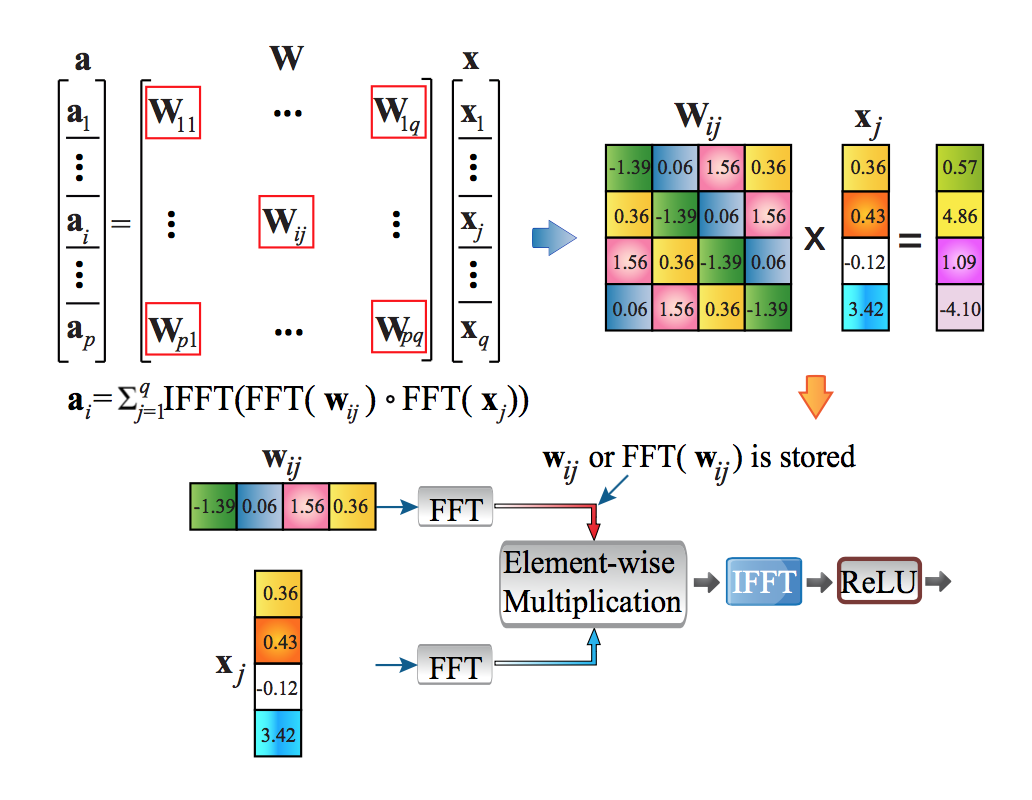
\includegraphics[width=0.8\linewidth]{Picture/forward.png}
		\caption{Illustration of the calculation of $W_{x}$ in the inference process}
		\label{Fig:1}
	\end{center}
	% \vspace{-0.1em}
\end{figure}

% \begin{eqnarray}
% 	% a_{5} &=& f\left( W_{51}\cdot X_{1}+W_{52}\cdot X_{2}+W_{53}\cdot X_{3}+W_{54}\cdot X_{4}\right)\\
% 	Y\left( x,y,p\right) =\sum ^{r}_{i=1}\sum ^{r}_{j=1}\sum ^{c}_{c=1}F\left( i,j,c,p\right) X\left( x+i-1,y+j-1,c\right)
% \end{eqnarray}

}
    
\frame{
\frametitle{Block-circulant matrices}%此页的标题

\begin{figure}
	\begin{center}
		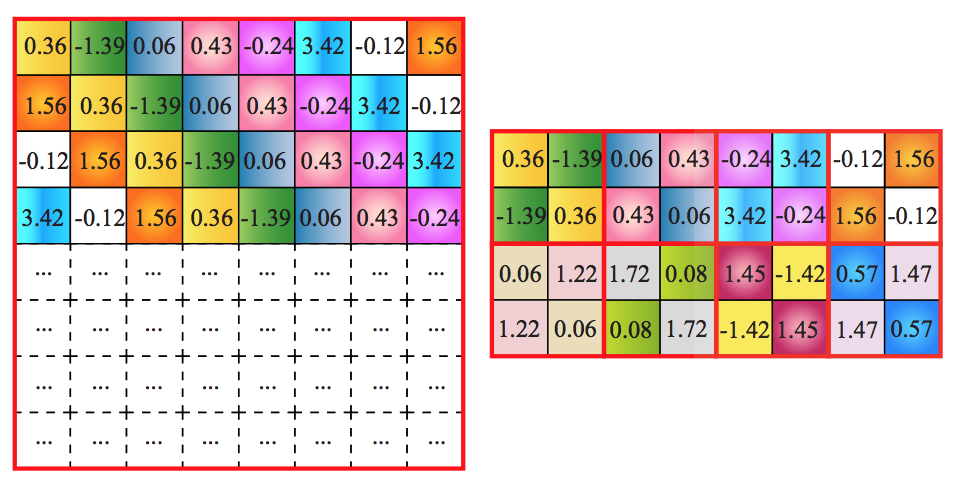
\includegraphics[width=0.8\linewidth]{Picture/block.png}
		\caption{when the numbers of inputs and outputs are not equal}
		\label{Fig:2}
	\end{center}
	% \vspace{-0.1em}
\end{figure}

% \begin{eqnarray}
% 	% a_{5} &=& f\left( W_{51}\cdot X_{1}+W_{52}\cdot X_{2}+W_{53}\cdot X_{3}+W_{54}\cdot X_{4}\right)\\
% 	Y\left( x,y,p\right) =\sum ^{r}_{i=1}\sum ^{r}_{j=1}\sum ^{c}_{c=1}F\left( i,j,c,p\right) X\left( x+i-1,y+j-1,c\right)
% \end{eqnarray}

}
    \frame{
\frametitle{Result}%此页的标题

\begin{figure}
	\begin{center}
		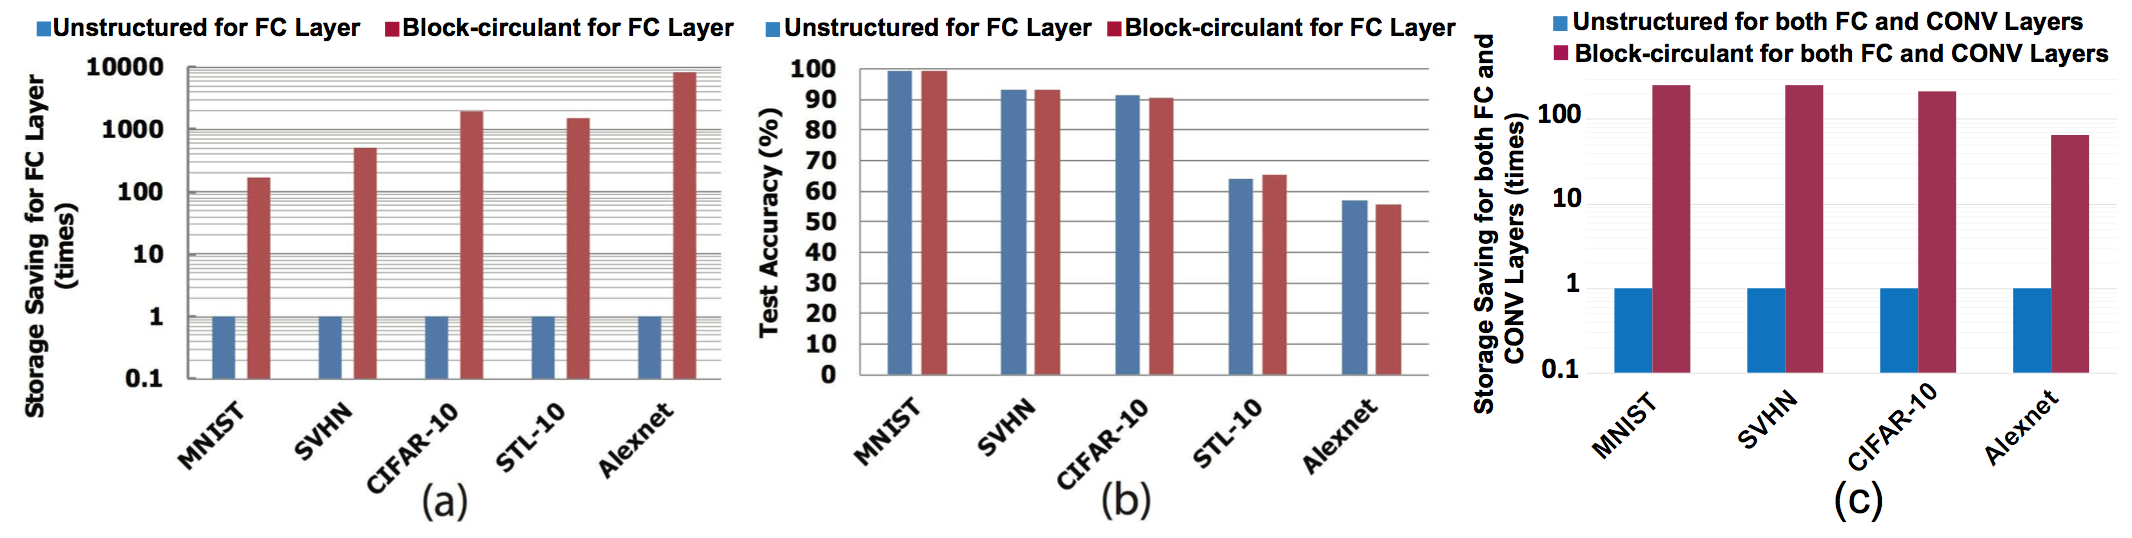
\includegraphics[width=1.01\linewidth]{Picture/result.png}
		\caption{(a) Storage saving and (b) test accuracy after using block-circulant FC layer for DCNN models on di erent datasets. (c) Storage saving after using both block-circulant FC layer and block-circulant CONV layer for DCNNs on MNIST, SVHN, CIFAR-10, and ImageNet datasets.}
		\label{Fig:3}
	\end{center}
	% \vspace{-0.1em}
\end{figure}

% \begin{eqnarray}
% 	% a_{5} &=& f\left( W_{51}\cdot X_{1}+W_{52}\cdot X_{2}+W_{53}\cdot X_{3}+W_{54}\cdot X_{4}\right)\\
% 	Y\left( x,y,p\right) =\sum ^{r}_{i=1}\sum ^{r}_{j=1}\sum ^{c}_{c=1}F\left( i,j,c,p\right) X\left( x+i-1,y+j-1,c\right)
% \end{eqnarray}

}


\end{document}

